\documentclass[19pt]{article}

\usepackage{arxiv}
\usepackage{makeidx}
\usepackage{fancyhdr}

\usepackage[utf8]{inputenc} % allow utf-8 input
\usepackage[T1]{fontenc}    % use 8-bit T1 fonts
\usepackage{hyperref}       % hyperlinks
\usepackage{url}            % simple URL typesetting
\usepackage{booktabs}       % professional-quality tables
\usepackage{graphicx}
\usepackage{amsfonts}       % blackboard math symbols
\usepackage{amsmath}
\usepackage{nicefrac}       % compact symbols for 1/2, etc.
\usepackage{microtype}      % microtypography
\usepackage{lipsum}

\pagestyle{fancy}
\title{AI in Medicine : Segmentation of Lymph tissues and localization of Cancer cells}


\author{
  Spandan Ghosh\thanks{Use footnote for providing further
    information about author (webpage, alternative
    address)---\emph{not} for acknowledging funding agencies.} \\
    Department of \emph{Electronics and Communication Engineering}\\
  Institute of Engineering \& Management\\
  Kolkata, India \\
  \texttt{spandanghosh2@gmail.com} \\
}
\begin{document}

\maketitle

\begin{abstract}
    Artificial Intelligence has been setting the benchmark for almost all commercial and research fields. Since the rapidly growing popularity of these approaches now draw the interests of the people in the resepective fields of application, we now define state of the art benchmarks with respect to how well several networks perform in different fields. Medical Imaging and the analysis of these images are no different. The polished techniques in Digital Image Processing such as the various filters, transforms, thresholding techniques have already been in use to reduce redundant human work when these techniques can perform pattern recognition for trivial, repititive tasks. The effect of the evolution of Deep Learning has allowed the learning of complex convolution filters using Convolutional Neural Networks(CNNs) which now permit the detection of intricate patterns and segmenting them to such an extent that these now become more efficient than the human eye in several cases. Medical Images however, post various challenges that are usually absent in other applications of Deep Learning in Computer Vision. 

    The first and primary issue is the quantity of data available. The amount of data available is nowhere close to the other real world applications such as classification of cusines by their snapshots. Moreover, medical images cannot be readily scraped or taken from the real world. Taking the problem at hand, one cannot simply step out into the world and acquire scanned and labelled images of Lymph Tissues. Their aquisition depends on Medical Institutions. Furthermore, the process of capturing, labelling, processing and releasing such a dataset is difficult and requires specialized attention from medical professionals. The second issue is that this, combined with the fact that expensive equipment may be required for their collection makes the process expensive.

    Segmentation adds another complexity:\textbf{The complexity of effort}. Segmentation involves a pixel to pixel mapping between the input and an output. Every single tissue sample image needs to be segmented by a medical expert for us to train an algorithm to do so automatically on other images. This process is tedious. In this project, along with reviewing certain approaches of interest, I am going to achive the a segmentation map on the input image without using a segmentation levels and am also going to discuss some alternative methods in which the above claimed can be achieved and when and where which should be preferred.
    
\keywords{Semantic Segmentation\and Medical Image Analysis \and Associative Networks \and Deep Learning}
\end{abstract}
\newpage
    \tableofcontents
\newpage
% keywords can be removed



\section{Introduction}
The upsurge in the dominance of Deep Learning in defining the Statei-of-the-Art in a great variety of fields. Both Research and Industrial organizations all over the world are on a lookout to capitalize on the edge provided by Deep Learning and to leverage an increase in performance or profit in accordance with the goals of the organization. With data being in abundance in this digital age and the greatly evolved compute capacity with the rise of GPUs (Graphical Processing Units), the tedious and compute hungry processing of training models on particular datasets has become easier and practically feasable.

\subsection{Motivation}
There has been a huge upsurge in the replacement of tedious and laborious work with algortihms to automate the process. Segmentation is no different. Segmentation is the process of reconstruction of an input image as the output image with certain pixels of the image highlighted or labelled to be of a particular class or to have a particular property. In Medical Imaging, this is quite often required in the highlighting of infected regions or affected areas in cells or scans. Before getting into the approaches in Digital Image Processing and Deep Learning to solve such problems, let us have a look at some typical segmentated images.

\begin{center}
    \begin{figure}[!h!t!b]
        \centerline{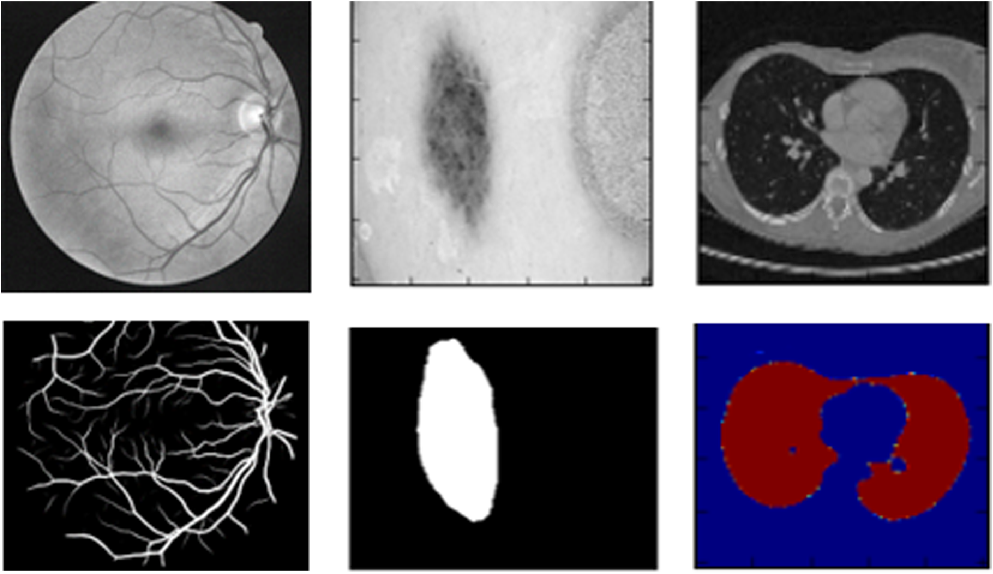
\includegraphics[width=105mm,height=65mm]{images/segs.png}}
        \caption{Some Segmented images}
        \label{fig:1}
    \end{figure}
\end{center}

Segmentation is p
\cite{kour2014real}

\bibliographystyle{unsrt}  

\bibliography{references}  %%% Remove comment to use the external .bib file (using bibtex).
%%% and comment out the ``thebibliography'' section.


%%% Comment out this section when you \bibliography{references} is enabled.

\end{document}
